
The next data structure we are going to consider is the queue. It is again a very simple data  structure, conceptually an array that is accessible from both ends: the data is added to the  end of the array and removed from the beginning of it. There are some very important  differences between the queue and the stack when it comes to implementation. There are  also many similarities, and we will refer to the previous section frequently. 

Just like the stack, the STL has a queue container, std::queue, and it has the exact  same problem when it comes to concurrency: the interface for removing elements is  not transactional, it requires three separate member function calls. If we wanted to use std::queue with a lock to create a thread-safe queue, we would have to wrap it just like we did with the stack:

\hspace*{\fill} \\ %插入空行
\noindent
\textbf{03\_queue.C}
\begin{lstlisting}[style=styleCXX]
template <typename T> class mt_queue {
	std::queue<T> s_;
	mutable spinlock l_;
	public:
	void push(const T& v) {
		std::lock_guard g(l_);
		s_.push(v);
	}
	std::optional<T> pop() {
		std::lock_guard g(l_);
		if (s_.empty()) {
			return std::optional<T>(std::nullopt);
		} else {
			std::optional<T> res(std::move(s_.front()));
			s_.pop();
			return res;
		}
	}
};
\end{lstlisting}

We decided to use the spinlock right away (a simple benchmark can confirm that it is again faster than a mutex). The front() method, if desired, can be implemented similarly to the pop() method, only without removing the front element. The basic benchmark again measured the time it takes to push an element onto the queue and pop it back. Using the same X86 machine we did in the last section, we can obtain these  numbers:

\hspace*{\fill} \\ %插入空行
\begin{center}
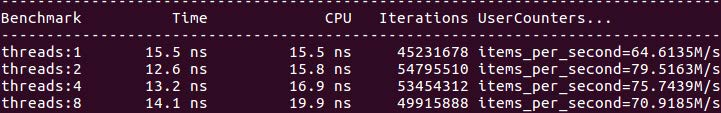
\includegraphics[width=0.9\textwidth]{content/2/chapter7/images/17.jpg}\\
Figure 7.17 – Performance of a spinlock-guarded std::queue
\end{center}

For comparison, on the same hardware, std::queue without any locks delivers about 280M items per second (an item is a push and a pop, so we measure how many elements we can send through the queue per second). So far, the picture is very similar to what we have seen earlier for the stack. To do better than the lock-guarded version, we have to try to come up with a lock-free implementation.

\subsubsubsection{7.4.1\hspace{0.2cm}Lock-free queue}

Before we dive into designing a lock-free queue, it is important to do a detailed analysis of each transaction, just like we did for the stack. Again, we will assume that the queue is built on top of an array or an array-like container (and we will defer the questions about what happens when the array is full). Pushing elements onto the queue looks just like it does for the stack: 

\hspace*{\fill} \\ %插入空行
\begin{center}
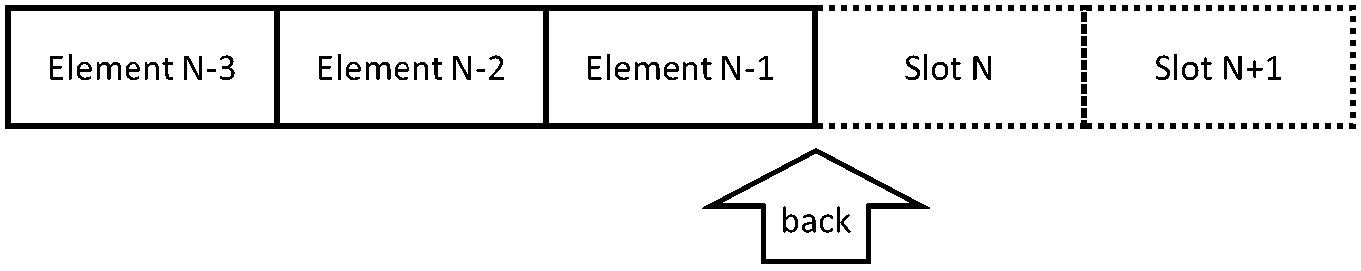
\includegraphics[width=0.9\textwidth]{content/2/chapter7/images/18.jpg}\\
Figure 7.18 – Adding elements to the back of the queue (producer's view)
\end{center}

All we need is the index of the first empty slot in the array. Removing elements from the queue, however, is quite different from the same operation on the stack. You can see this  in Figure 7.19 (compare it with Figure 7.9):

\hspace*{\fill} \\ %插入空行
\begin{center}
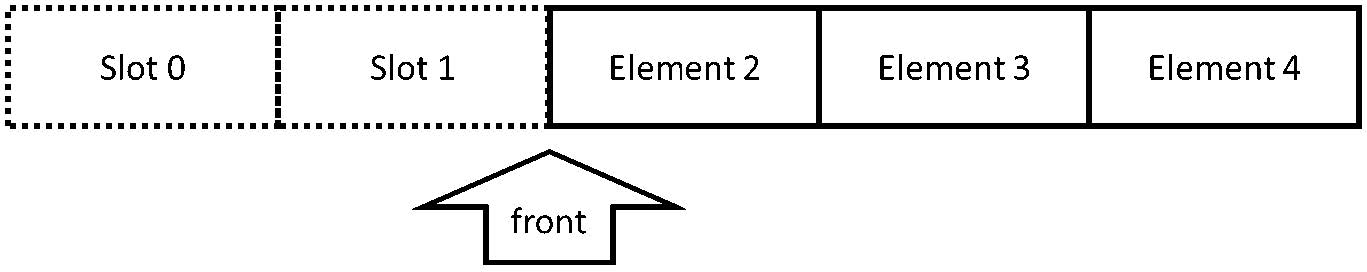
\includegraphics[width=0.9\textwidth]{content/2/chapter7/images/19.jpg}\\
Figure 7.19 – Removing elements from the front of the queue (consumer's view)
\end{center}

The elements are removed from the front of the queue, so we need the index of the first element that has not been removed yet (the current front of the queue), and that index is also advanced. 

Now we come to the crucial difference between the queue and the stack: in the stack, both producer and consumer operate on the same location: the top of the stack. We have seen the consequences of this: once the producer started to construct a new element at the top of the stack, the consumer has to wait for it to complete. The pop operation cannot return the last constructed element without leaving a hole in the array, and it can't return the element being constructed until the construction is done.

The situation is very different for the queue. As long as the queue is not empty, the producers and the consumers do not interact at all. The push operation does not need to know what the front index is, and the pop operation does not care where the back index is as long as it's somewhere ahead of the front. The producers and the consumers are not competing for access to the same memory location. 

Whenever we have the case that there are several different ways to access the data structure and they (mostly) do not interact with each other, the general suggestion is to first consider the scenario where these roles are assigned to different threads. The further simplification can be to start with the case of one thread of each kind; in our case, it means one producer thread and one consumer thread. 

Since only the producer needs access to the back index, and there is only one producer thread, we don't even need an atomic integer for this index. Similarly, the front index is just a regular integer. The only time the two threads interact with each other is when the queue becomes empty. For that, we need an atomic variable: the size of the queue. The producer constructs the new element in the first empty slot and advances the back index (in any order, there is only one producer thread). Then, it increments the size of the queue to reflect the fact that the queue now has one more element ready to be taken from it. 

The consumer must operate in reverse order: first, check the size to make sure the queue is not empty. Then the consumer can take the first element from the queue and advance the front index. Of course, there is no guarantee that the size does not change between the time it is checked and the time the front element is accessed. But it does not cause any problems: there is only one consumer thread, and the producer thread can only increment the size. 

While exploring the stack, we deferred the issue of adding more memory to the array and assumed that we somehow know the maximum capacity of the stack and will not exceed it (we could also make the push operation fail if that capacity is exceeded). For the queue, the same assumption is not enough: as the elements are added and removed from the queue, both the front and the back indices advance and will eventually reach the end of the array. Of course, at this point, we have the first elements of the array unused, so the simplest solution is to treat the array as a circular buffer and use modulo arithmetic for array indices:

\hspace*{\fill} \\ %插入空行
\noindent
\textbf{03a\_atomic\_pc\_queue.C}
\begin{lstlisting}[style=styleCXX]
template <typename T> class pc_queue {
	public:
	explicit pc_queue(size_t capacity) : 
	capacity_(capacity),
	data_(static_cast<T*>(::malloc(sizeof(T)*capacity_))) {}
	~pc_queue() { ::free(data_); }
	bool push(const T& v) {
		if (size_.load(std::memory_order_relaxed) >= capacity_)
		return false;
		new (data_ + (back_ % capacity_)) T(v);
		++back_;
		size_.fetch_add(1, std::memory_order_release);
		return true;
	}
	std::optional<T> pop() {
		if (size_.load(std::memory_order_acquire) == 0) {
			return std::optional<T>(std::nullopt);
		} else {
			std::optional<T> res(
			std::move(data_[front_ % capacity_]));
			data_[front_ % capacity_].~T();
			++front_;
			size_.fetch_sub(1, std::memory_order_relaxed);
			return res;
		}
	}
private:
const size_t capacity_;
T* const data_;
size_t front_ = 0;
size_t back_ = 0;
std::atomic<size_t> size_;
};
\end{lstlisting}

This queue requires a special benchmark because of the constraints we accepted on its design: one producer thread and one consumer thread:

\hspace*{\fill} \\ %插入空行
\noindent
\textbf{03a\_atomic\_pc\_queue.C}
\begin{lstlisting}[style=styleCXX]
pc_queue<size_t> q(1UL<<20);
void BM_queue_prod_cons(benchmark::State& state) {
	const bool producer = state.thread_index & 1;
	const size_t N = state.range(0);
	for (auto _ : state) {
		if (producer) {
			for (size_t i = 0; i < N; ++i) q.push(i);
		} else {
			for (size_t i = 0; i < N; ++i) 
			benchmark::DoNotOptimize(q.pop());
		}
	}
	state.SetItemsProcessed(state.iterations()*N);
}
BENCHMARK(BM_queue_prod_cons)->Arg(1)->Threads(2)
->UseRealTime();
BENCHMARK_MAIN();
\end{lstlisting}

For comparison, we should benchmark our lock-guarded queue under the same conditions (performance of the locks is generally sensitive to the exact nature of the contention between threads). On the same X86 machine, the two queues perform at roughly the same throughput of 100M integer elements per second. On the ARM processor, the locks are relatively more expensive, in general, and our queue is no exception:

\hspace*{\fill} \\ %插入空行
\begin{center}
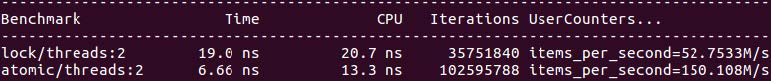
\includegraphics[width=0.9\textwidth]{content/2/chapter7/images/20.jpg}\\
Figure 7.20 – Performance of a lock-based versus a lock-free queue of integers on ARM
\end{center}

However, even on X86, our analysis is not yet complete. In the previous section, we mentioned that if the stack elements are large, copying them takes relatively longer than the thread synchronization (locking or atomic operations). We could not make much use of it because most of the time, one thread still had to wait for the other thread to complete the copy, so the alternative was suggested: a stack of pointers, with the actual data stored elsewhere. The downside is that we need another thread-safe container to store this data (although often, the program needs to store it somewhere anyway). This is still a viable suggestion for the queue, but now we have another alternative. As we have already mentioned, the producer and consumer threads in the queue do not wait for each other: their interaction ends after the size is checked. It stands to reason that, if the data elements are large, the lock-free queue will have an advantage because both threads can copy the data at the same time and the contention between the threads, or the time when two threads are competing for access to the same memory location (the lock or the atomic value), is much shorter. To do such a benchmark, we just need to create a queue of large objects, such as a struct with a large array in it. As expected, the lock-free queue now performs faster, even on the X86 hardware:

\hspace*{\fill} \\ %插入空行
\begin{center}
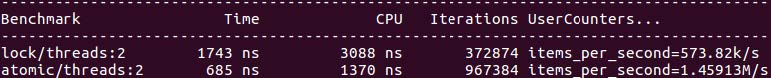
\includegraphics[width=0.9\textwidth]{content/2/chapter7/images/21.jpg}\\
Figure 7.21 – Performance of a lock-based versus a lock-free queue of large elements on X86
\end{center}

Even with the restrictions we have imposed, this is a very useful data structure: this queue can be used for transferring data between a producer and a consumer thread when we know an upper bound on the number of elements we can enqueue or can handle the situation when the producer has to wait before pushing more data. The queue is very efficient; even more important for some applications is the fact that it has very low and predictable latency: the queue itself is not just lock-free but wait-free. One thread never has to wait for the other unless the queue is full. By the way, if the consumer has to do certain processing on each data element it takes from the queue and starts falling behind until the queue fills up, one common approach is to have the producer process the elements it could not enqueue. This serves to delay the producer thread until the consumer can catch up (this method is not suitable for every application since it can process data out of order, but quite often, it works).

The generalization of our queue for the case of many producer or consumer threads is going to make the implementation more complex. The simple wait-free algorithm based on atomic size no longer works even if we make the front and back indices atomic: if multiple consumer threads read a non-zero value of size, this is no longer sufficient for all of them to proceed. With multiple consumers, the size can decrease and become zero after it was checked by one thread and found to be non-zero (it just means that the other threads popped all remaining elements after the first thread tested the size, but before it tried to access the front of the queue).

One general solution is to use the same technique we used for the stack: pack the front and back indices into a single 64-bit atomic word and access them both atomically using compare-and-swap. The implementation is similar to that of the stack; the reader who understood the code in the previous section is well-prepared to implement this queue. There are other lock-free queue solutions that can be found in the literature; this chapter should give you sufficient background to understand, compare, and benchmark these implementations.

Implementing a complex lock-free data structure correctly is a time-consuming project that requires skill and attention. It is good to have some performance estimates before the implementation is complete, so we can know whether the effort is likely to pay off. We have already seen one approach to benchmarking the code that does not yet exist: a simulated benchmark that combines the operations on a non-thread-safe datastructure (local to eachthread) with the operations on shared variables (locks or atomic data). The goal is to come up with a computationally equivalent code fragment that can be benchmarked; it is never going to be perfect, but if we have an idea for a lock-free queue with three atomic variables and a compare-and-swap operation on each one, and we discover that the estimated benchmark is several times slower than the spinlock-guarded queue, the work of implementing the real queue is unlikely to pay off.

The second way to benchmark partially implemented code is to construct benchmarks that avoid certain corner cases that we have not yet implemented. For example, if you expect the queue to not be empty most of the time, and your initial implementation does not handle the case of the empty queue, you should benchmark that implementation and restrict the benchmark so the queue never gets empty. This benchmark will tell you if you are on the right track: it will show what performance you can expect in the typical case of the non-empty queue. We had actually taken this approach already when we deferred handling of the case when the stack or the queue runs out of memory. We simply assumed that it's not going to happen very often and constructed the benchmark to avoid this case.

There is yet another type of concurrent data structure implementation that can often be very efficient. We are going to learn about this technique next.

\subsubsubsection{7.4.2\hspace{0.2cm}Non-sequentially consistent data structures}

Let's first revisit the simple question, what is a queue? Of course, we know what a queue is: it's a data structure such that the element added first is also retrieved first. Conceptually, and in many implementations, this is guaranteed by the order in which the elements are added to the underlying array: we have an array of queued elements, new entries are added to the front, while the oldest ones are read from the back.

But let's examine closely if this definition still holds for a concurrent queue. The code that is executed when an element is read from the queue looks something like this:

\begin{lstlisting}[style=styleCXX]
T pop() {
	T return_value;
	return_value = data[back];
	--back;
	return return_value;
}
\end{lstlisting}

The return value may be wrapped in std::optional or passed by reference; it doesn't matter. The point is, the value is read from the queue, the back index is decremented, and the control returns to the caller. In a multi-threaded program, the thread can be preempted at any moment. It is entirely possible that if we have two threads, A and B, and thread A reads the oldest element from the queue, it is thread B that completes execution of pop() first and returns its value to the caller. Thus, if we enqueue two elements X and Y, in that order, and have multiple threads dequeue them and print their values, the program prints Y then X. The same kind of reordering can happen when multiple threads push elements onto the queue. The end result is that even if the queue itself maintains a strict order (if you were to pause the program and examine the array in memory, the elements are in the right order), the order of dequeued elements as observed by the rest of the program is not guaranteed to be exactly the order in which they were enqueued.

Of course, the order is not entirely random either: even in a concurrent program, a stack looks very different from a queue. The order of the data retrieved from a queue is approximately the order in which the values were added; significant rearrangements are rare (they happen when one thread is, for some reason, delayed for a significant time).

There is another very important property that is still preserved by our queue: sequential consistency. A sequentially consistent program produces the output that is identical to the output of a program where operations from all threads are executed one at a time (without any concurrency), and the order of the operations executed by any particular thread is not changed. In other words, the equivalent program takes the sequences of operations executed by all threads and interleaves them but does not reshuffle them. 

Sequential consistency is a convenient property to have: it is much easier to analyze the behavior of such programs. For example, in the case of the queue, we have the guarantee that if two elements X and Y were enqueued by thread A, X first, then Y, and they happen to be both dequeued by thread B, they will come out in the correct order. On the other hand, we can argue that, in practice, it doesn't really matter: the two elements may be dequeued by two different threads, in which case they can appear in any order, so the program has to be able to handle it. 

If we are willing to give up sequential consistency, this opens up a whole new approach to designing concurrent data structures. Let's explore it on the example of a queue. The basic idea is this: instead of a single queue thread-safe queue, we can have several single-threaded sub-queues. Each thread must atomically acquire exclusive ownership of one of these sub-queues. The simplest way to implement this is with an array of atomic pointers to the sub-queues, as shown in Figure 7.22. To acquire the ownership and, at the same time, prevent any other thread from getting access to the queue, we atomically exchange the sub-queue pointer with null.

\hspace*{\fill} \\ %插入空行
\begin{center}
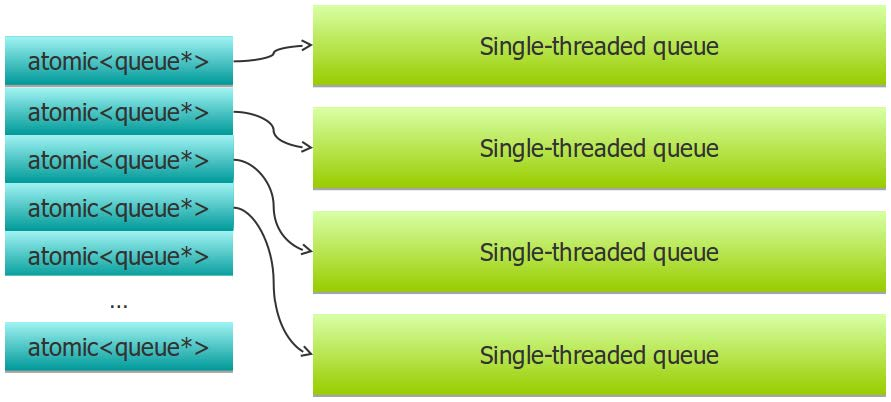
\includegraphics[width=0.9\textwidth]{content/2/chapter7/images/22.jpg}\\
Figure 7.22 – Non-sequentially-consistent queue based on an array sub-queue accessed via atomic 
pointers
\end{center}

A thread that needs to access the queue must first acquire a sub-queue. We can start from any element of the pointer array; if it's null, that sub-queue is currently busy, and we try the next element, and so on until we reserve a sub-queue. At this point, there is only one thread operating on the sub-queue, so there is no need for thread safety (the sub-queue can even be std::queue). After the operation (push or pop) is completed, the thread returns the ownership of the sub-queue to the queue by atomically writing the sub-queue pointer back into the array.

The push operation must continue to try to reserve the sub-queue until it finds one (alternatively, we can allow the push to fail after a certain number of tries and signal the caller that the queue is too busy). The pop operation may reserve a sub-queue only to find that it's empty. In this case, it has to try to pop from another sub-queue (we can keep an atomic count of elements in the queue to optimize the fast return if the queue is empty).

Of course, pop may fail on one thread and report that the queue is empty when in fact, it isn't because another thread has pushed new data onto the queue. But this could happen with any concurrent queue: one thread checks the queue size, finds that the queue is empty, but before the control is returned to the caller, the queue becomes non-empty. Again, the sequential consistency puts some limits on what kind of inconsistencies can be observed by multiple threads, while our non-sequentially consistent queue makes the order of outgoing elements much less certain. Still, the order is maintained on average. 

This is not the right data structure for every problem, but when the mostly queue-like most of the time order is acceptable, it can lead to significant performance improvements, especially in systems with many threads. Observe the scaling of the non-sequentially consistent queue on a large X86 server running many threads:

\hspace*{\fill} \\ %插入空行
\noindent
\textbf{03b\_noncst\_queue.C}
\begin{center}
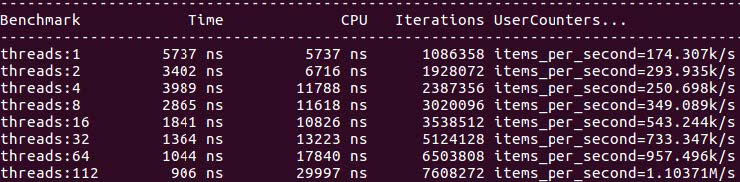
\includegraphics[width=0.9\textwidth]{content/2/chapter7/images/23.jpg}\\
Figure 7.23 – Performance of the non-sequentially-consistent queue
\end{center}

In this benchmark, all threads do both push and pop operations, and the elements are fairly large (copying each element requires copying 1KB of data). For comparison, the spinlock-guarded std::queue delivers the same performance (about 170k elements per second) on a single thread but does not scale at all (the entire operation is locked), and the performance drops slowly (due to the overhead of locking) to about 130k elements per second for the maximum number of threads.

Of course, many other data structures can benefit from this approach if you're willing to embrace the chaos of the non-sequentially-consistent programs for the sake of 
performance. 

The last subject we need to cover when it comes to concurrent sequential containers such as stack and queue is how to handle the situation when they need more memory

\subsubsubsection{7.4.3\hspace{0.2cm}Memory management for concurrent data structures}

So far, we persisted in pushing back on the issue of memory management and assumed that the initial memory allocation for the data structure would suffice, at least for lock-free data structures that do not make the entire operation single-threaded. The lock-guarded and the non-sequentially-consistent data structures we have seen throughout this chapter do not have this problem: under the lock or exclusive ownership, there is only one thread operating on the particular data structure, so the memory is allocated in the usual way.

For a lock-free data structure, memory allocation is a significant challenge. It is usually a relatively long operation, especially if the data must be copied to the new location. Even though multiple threads may detect that the data structure ran out of memory, usually only one thread can add new memory (it is very hard to make that part multi-threaded as well), the remaining threads must wait. There is no good general solution to this problem, but we will present several recommendations.

First of all, the best option is to avoid the problem altogether. In many situations, when a lock-free data structure is needed, it is possible to estimate its maximum capacity and preallocate the memory. For example, we may know the total number of data elements we are going to enqueue. Alternatively, it may be possible to push the problem back to the caller: instead of adding memory, we can tell the caller that the data structure is out of capacity; in some problems, this may be an acceptable trade-off for the performance of the lock-free data structure.

If the memory needs to be added, it is highly desirable that adding memory should not require copying of the entire existing data structure. This implies that we can't simply allocate more memory and copy everything to the new location. Instead, we must store the data in memory blocks of a fixed size, the way std::deque does it. When more memory is required, another block is allocated, and there are usually a few pointers that need to be changed, but no data is copied. 

In all cases where memory allocation is done, this must be an infrequent event. If this is not so, then we are almost certainly better off with a single-threaded data structure protected by a lock or temporary exclusive ownership. The performance of this rare event is not critical, and we can simply lock the entire data structure and have one thread do the memory allocation and all the necessary updates. The key requirement is to make the common execution path, the one where we do not need more memory, as fast as possible. 

The idea is very simple: we certainly do not want to acquire the memory lock on every thread every time, which would serialize the whole program. We also don't need to do this: most of the time, we are not out of memory, and there is no need for this lock. So instead, we are going to check an atomic flag. The flag is set only if memory allocation is currently in progress, and all threads must wait:

\begin{lstlisting}[style=styleCXX]
std::atomic<int> wait; // 1 if managing memory
if (wait == 1) {
	… wait for memory allocation to complete …
}
if ( … out of memory … ) {
	wait = 1;
	… allocate more memory …
	wait = 0;
}
… do the operation normally … 
\end{lstlisting}

The problem here is that multiple threads may detect the out-of-memory condition at the same time before one of them sets the wait flag; they would then all try to add more memory to the data structure. This usually creates a race (reallocating the underlying storage is rarely thread-safe). However, there is a simple solution known as the double-checked locking. It uses both a mutex (or another lock) and an atomic flag. If the flag is not set, all is well, and we can proceed as usual. If the flag is set, we must acquire the lock and check the flag again:

\begin{lstlisting}[style=styleCXX]
std::atomic<int> wait;  // 1 if managing memory
std::mutex lock;
while (wait == 1) {};  // Memory allocation in progress
if ( … out of memory … ) {
	std::lock_guard g(lock);
	if (… out of memory …) { // We got here first!
		wait = 1;
		… allocate more memory …
		wait = 0;
	}
}
… do the operation normally …
\end{lstlisting}

The first time, we check the out-of-memory condition without any locking. It is fast and, most of the time, we are not out of memory. The second time, we check it under the lock, where we have the guarantee that only one thread is executing at a time. Multiple threads may detect that we are out of memory; however, the first one to get the lock is the thread that handles this case. All remaining threads wait for the lock; when they acquire the lock, they do the second check (hence, double-checked locking) and discover that we are no longer out of memory. 

This approach can be generalized to handle any special case that happens very infrequently but is much more difficult to implement in a lock-free manner than the rest of the code. In some cases, it may even be useful for situations such as the empty queue: as we have seen, the handling of multiple producers or multiple consumers would require a simple atomically incremented index if the two groups of threads never had to interact with each other. If, in a particular application, we have a guarantee that the queue rarely, if ever, becomes empty, we could favor an implementation that is very fast (wait-free) for the non-empty queue but falls back on a global lock if the queue might be empty.

We have covered the sequential data structures in enough detail now. It is time to study the nodal data structures next. 






























